\section{Discussion}
\label{sec:evaluation}
\todo[inline]{CDC: MISSING:
Nella evaluation, dobbiamo riportare
1) la memoria usata e
2) il tempo richiesto dall'algoritmo per fare (a) merge e (b) elaborazione. Se potessimo mostrare un grafico che illustra come la memoria richiesta aumenta pian pianino mentre si raccolgono i pezzi di log e infine quanta ne serva per l'elaborazione (parlo solo della memoria riservata in TEE) sarebbe ancora meglio. L'uso di memoria qui conta perché è un parametro fondamentale.
\\
Dobbiamo informare il lettore sulle caratteristiche del log (numero eventi, numero tracce, dimensione totale in KB una volta salvato in formato XES), come lo abbiamo creato, perché il modello non è uguale a quello di Fig. 1.
}

In the preceding section, we expounded upon the functioning of the secure event log sharing mechanism through the use of a Trusted Execution Environment (TEE). In order to determine the robustness and effectiveness of the framework, it is important to thoroughly evaluate diverse requirements of its operation.
Of particular significance is the assessment of the accuracy and reliability of the event log generated through the amalgamation of logs received from disparate providers. This evaluation is pivotal in establishing the efficacy of the collaborative data exchange process. The primary objective the \cref{sec:evaluation} is to delve into a convergence analysis by evaluating the precision and structure of the Petri Net 
\todo{CDC: This is not a Petri net but a Workflow net. Not the same thing.}
derived from the merged event log with that of the Petri Net originating from the individual event logs. This comparison serves as a critical means to gauge the reliability of the generated process model and the extent to which it accurately represents the collaborative workflow. We then took into analysis other requirements such as integrity and confidentiality in \cref{sec:evaluation} and validation on real data in \cref{sec:evaluation}.
\todo{CDC: We should give the numbers of the subsections, not the section here. Otherwise, it is always Section~\ref{sec:evaluation} mentioned all over the place.}

\subsection{Validation}
We conducted a practical validation of our framework using the BPIC 2013 dataset,
\todo{CDC: Missing: citation}
specifically the Volvo IT incident management system event log. As this log pertains to an intra-company setting, we strategically filtered via ProM the data to isolate department-specific segments. This allowed us to rigorously test the functionality of our framework by securely exchanging partial logs, effectively simulating an inter-organizational context


\subsection{Convergence}

\begin{figure}[t]
\centering
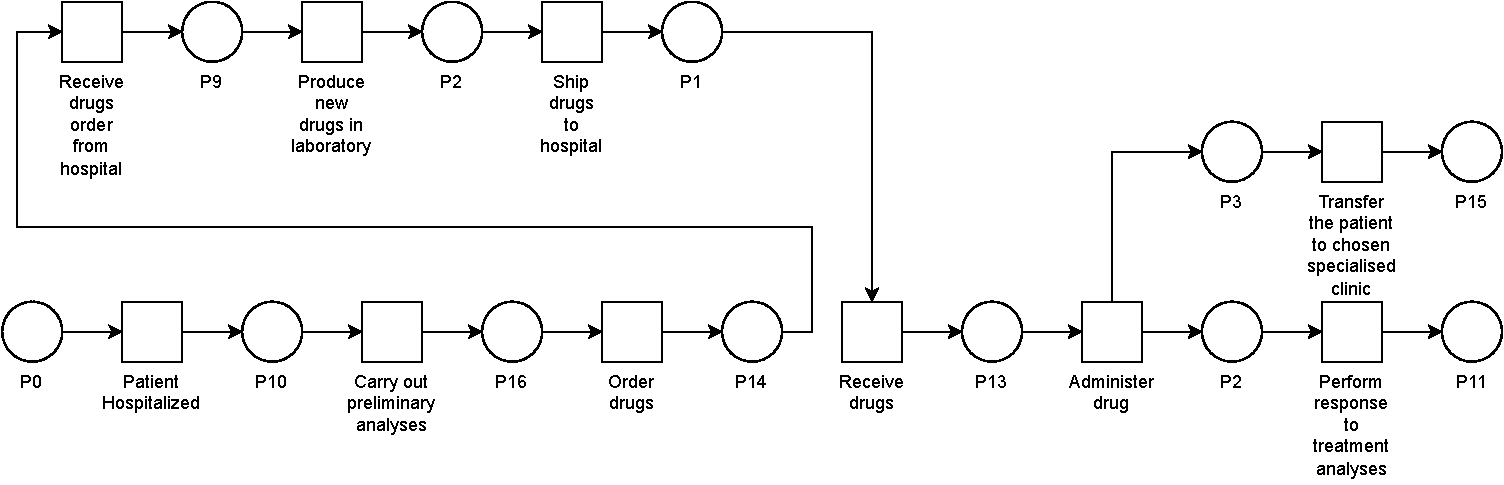
\includegraphics[width= 0.9\linewidth]{content/figures/mergedpetri.pdf}
\caption{Workflow Net generated from the merged event log}
\label{fig:merged_petri}
\end{figure}

Matching the two Workflow Nets reveals how their convergence substantiates the efficacy and adequacy of the event log sharing mechanism. The first Workflow Net is crafted from the merged event log, which encapsulates the collective data from the hospital, specialised clinc and the pharmaceutical company. The second Workflow Net originates from the unaltered entire event log. This comparative study aims to elucidate the congruence and comparability of these two Workflow Nets.
Upon visual examination, it is possible to notice that the Workflow Net originating from the merged event log closely mirrors the structure and behavior of the Workflow Net derived from the individual event logs. The markings, transitions, and places within both Workflow Nets exhibit a remarkable congruence, indicative of a shared underlying process model. This congruence further extends to the temporal sequencing of events and the causal relationships among process steps. This substantial resemblance between the two Workflow Nets serves as a testament to the seamless convergence of disparate event logs, achieved through the secure exchange mechanism. The fact that the collaborative process model, represented by the Workflow Net generated from the merged event log, aligns closely with the independent models of individual organizations underscores the fidelity and accuracy of the data exchange process.
\subsection{Integrity and Confidentiality}
An essential aspect of the evaluation pertains to the fundamental principles of integrity and confidentiality upheld by the Trusted Execution Environment (TEE), crucial pillars that underpin the effectiveness and trustworthiness of the event log sharing mechanism. In this framework, the TEE is the cornerstone of data processing, demonstrating praiseworthy abilities to ensure data integrity. Throughout the entire process, from the moment data is ingested from individual organizations to the merging of event logs, the TEE maintains an unyielding grip on data integrity, steadfastly safeguarding against unauthorized modifications. This veracity is established through cryptographic hashing and secure storage mechanisms that ensure that the merged event log remains unaltered and representative of the original data. Concurrent with data integrity, the TEE exercises a robust commitment to confidentiality. The cryptographic measures implemented within the TEE ensure that all data, whether in transit or at rest, is encrypted with a level of security that mitigates the risk of unauthorized access. This cryptographic fortification guarantees that sensitive information encapsulated within event logs remains comprehensively shielded, rendering them inaccessible to any unauthorized entities. As a result, participating organizations can confidently share their event logs, knowing that their proprietary and sensitive information remains impervious to prying eyes.

